\section{Experiment 3. Initial information and tradeoff of exploration}\label{sec:controlled}
Experiment 2 shows how changing search policies can affect discovery and refinement. We now test how their value depends on the information available at the start. The prediction is that global probes should be most useful when observations support the inferior basin A, whereas local concentration should be most useful when they already identify B.

At \(c=30\), each of 50 seeds has eight common background points outside the unit disks around both minima. Four additional points lie at radii \(0.35,0.39,0.43,0.47\) around either A or B, using the same randomly rotated directions in both designs. The initial best values are therefore \(1.1225\) near A and \(0.1225\) near B. All 12 observations count towards the budget, leaving 38 evaluations. Every near-B design has already attained discovery and core entry, but none has attained precision.

Standard BO-EI and BO-EI with probes fit to the same 12 observations and differ only by the ten-probe, as given Section~\ref{sec:bo_recovery}. Both CMA-ES variants initialise their means at the best observed point and use the same default population size and adaptation rules. They differ only in normalised initial step size: \(\sigma_0=0.25\) or \(0.05\), where bigger step size encourages exploration. Note that both variants subsequently adapt their step sizes. 

\begin{table}[!htb]
 \centering
 \caption{Experiment 3: attainment counts out of 50 runs}
 \label{tab:controlled}
 \begin{tabular}{lrrrr}
 \toprule
 & \multicolumn{3}{c}{Initial design near A} & Near B\\
 \cmidrule(lr){2-4}\cmidrule(l){5-5}
 Method & Discovery & Refinement near A & Precision & Precision\\
 \midrule
 Standard BO-EI            & 1  & 50 & 0 & 42\\
 BO-EI + probes            & 16 & 48 & 5 & 36\\
 CMA-ES, \(\sigma_0=0.25\) & 5 & 7 & 0 & 4\\
 CMA-ES, \(\sigma_0=0.05\) & 0 & 46 & 0 & 46\\
 \bottomrule
 \end{tabular}
\end{table}

Near A, probes increase BO-EI discovery from \(1/50\) to \(16/50\), a paired difference of 30 percentage points (95\% CI \([8.1,46.6]\)); five probe runs also attain precision (Table~\ref{tab:controlled}). Standard BO-EI refines near A in all 50 runs, showing that accurate local optimisation can coexist with failure to discover the better
region. 

Near B, standard BO-EI attains precision in \(42/50\) runs, compared with \(36/50\) with probes. Median terminal regret increases from \(0.00190\) to \(0.00495\). This illustrates the exploration-exploitation tradeoff, where probes consume evaluations that could otherwise refine a known promising region.

In the near-B experiment, reducing the initial CMA-ES scale raises precision from \(4/50\) to \(46/50\), a paired increase of 84 percentage points (95\% CI \([60.6,93.7]\)). The fraction of continuation evaluations inside the radius-0.5 core increases from \(5.9\%\) to \(75.6\%\), or approximately 2.3 versus 28.7 of the 38 available evaluations per run. At the larger scale, median terminal regret remains at the initial value of \(0.1225\), despite the supplied point already lying in the core. This supports the explanation that access to a good point is insufficient when subsequent sampling is poorly concentrated around it.

Near A, the same reduction increases refinement around the inferior minimiser from \(7/50\) to \(46/50\), while discovery changes from
\(5/50\) to \(0/50\). Smaller scale therefore improves local refinement at either starting location, but only refinement near B achieves the global precision target. These results explain why the scale and adaptation changes in Experiment 2 for CMA do not have a universal benefit: their consequences depend on which region receives more evaluations.

\begin{figure}[!htb]
 \centering
 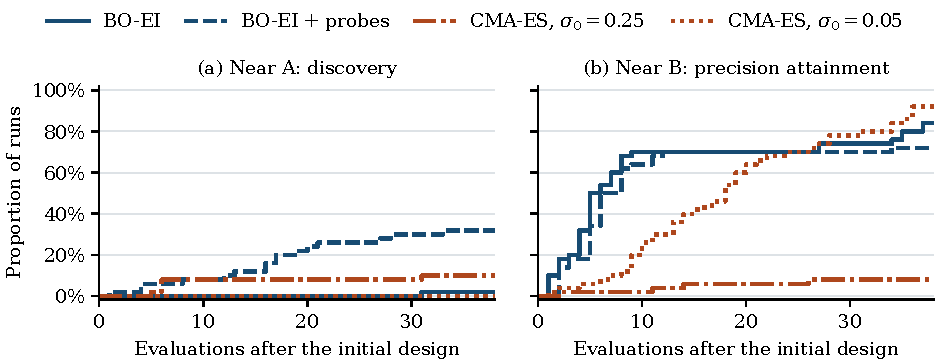
\includegraphics[width=.84\linewidth]{controlled_hits.pdf}
 \caption{Target attainment after the 12-evaluation initial design in Experiment 3. The near-A panel measures discovery, and the near-B panel measures precision.}
 \label{fig:controlled}
\end{figure}

Figure~\ref{fig:controlled} illustrates clearly the tradeoff of methods that favour exploration. Note that for methods such that BO with probes or CMA with larger $\sigma_0$ which prefer exploration, the methods often report a better ability to find the global minimum, but taken at a cost that when it reaches the optimum basin, they are less likely to find the actual minimum. Taken with Experiment 2, the evidence supports a dependence of the performance of methods on search location.